\subsection{Decision 3: Routes management}

\subsection*{Status}
Accepted.

\subsection*{Architectural Summary}
\begin{tabular}{|p{3.5cm}|p{10.5cm}|}
    \hline
    \textbf{In the context of} & Allowing terminals to present route options to passengers when they select their departure and arrival stations, \\
    \hline
    \textbf{Facing} & The challenge of letting passengers choose between different travel combination involving multiple tycoons, \\
    \hline
    \textbf{To achieve} & Streamlined integration with multiple tycoon systems, and accurate representation of options based on multiple factors, \\
    \hline
    \textbf{We considered} & Option 1: Direct Tycoon Integration; Option 2: Centralized Route Management Module; \\
    \hline
    \textbf{And decided for} & Option 2: Centralized Route Management Module \\
    \hline
    \textbf{Because} & It simplifies data flow and integration between the TRiP system and tycoon's systems, it improves scalability and maintainability of the system, \\
    \hline
    \textbf{Accepting} & Initial development effort and potential difficulties in data synchronization across modules. \\
    \hline
\end{tabular}

\subsection*{Concern}
The concern is to facilitate a seamless travel planning experience for passengers by ensuring the system can accurately and efficiently gather available route options and present them based on the user's criteria of price, time, and subscription status.
Related user stories are listed here:
\begin{itemize}
    \item \textbf{User Story 16:} As a passenger, I want to be able to purchase a single ticket that allows me to travel across all train networks so that I can travel seamlessly without needing to buy separate tickets for each tycoon's network.
    \item \textbf{User Story 26:} As a station manager, I want the system to offer real-time updates on train schedules and network disruptions so that I can keep passengers informed and manage station flow effectively.
\end{itemize}

\subsection*{Context}
The TrIP system needs to be able to compute optimized travel options (for instance best prices and lowest travel times), gathering information from multiple tycoon systems in order to align with passenger preferences and existing subscriptions.
The decision is centered on the system's interface with tycoon systems to retrieve and optimize route data, which impacts the functionality and performance of the terminal's route planning features for the passengers.

\subsection*{Criteria}
The key criteria for the decision include:
% mention usability
\begin{itemize}
    \item User-friendly passenger interface.
    \item Comprehensive and diverse route options.
    \item Accurate representation of options based on multiple factors.
    \item Streamlined integration with multiple tycoon systems.
\end{itemize}

\subsection*{Option 1: Direct Tycoon Integration}
Terminals directly interface with each tycoon system and the central database to collate route options. The route optimizer processes this data to present optimal travel solutions. This requires our system to have APIs to query each of the tycoons systems.
\begin{figure}[ht]
    \centering
    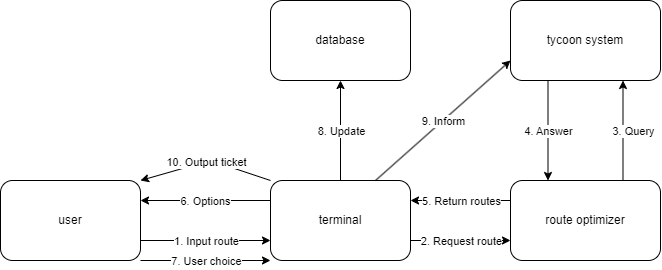
\includegraphics[width=\textwidth]{drawings/decision3_drawings/direct.png}
    \caption{Direct Data Management Interface}
    \label{fig:direct-data-interface}
\end{figure}

\subsection*{Option 2: Centralized Route Management Module}
A central route data management module acts as an intermediary between terminals and tycoon systems, standardizing and aggregating data before it is processed by the route optimizer. A database containing the timetables will be kept up to date by the tycoon (possibly though an API, this will be the focus of a later decision). The route data management system might cache optimized routes, in order to minimize database requests. A module specialized in running optimizations with the data it is provided with interacts solely with the Route Management Module.
\begin{figure}[ht]
    \centering
    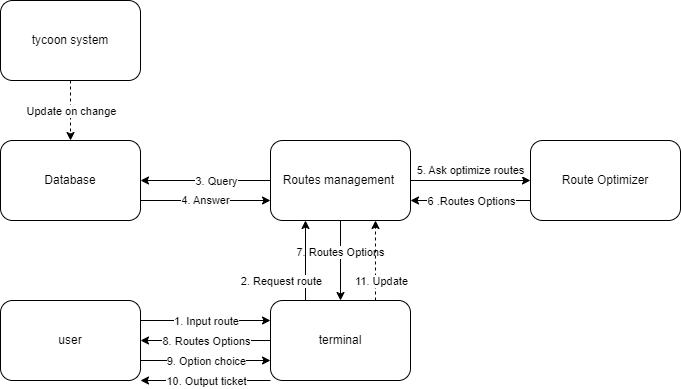
\includegraphics[width=\textwidth]{drawings/decision3_drawings/centralized.png}
    \caption{Centralized Route Management Module. Dashed lines represents steps to be explained in future decisions.}
    \label{fig:centralized-data-interface}
\end{figure}
  
\subsection*{Decision}
We have decided to proceed with Option 2: Centralized Route Management Module. This decision is based on the module's ability to simplify the data flow between systems and to effectively manage the complexity of integrating with multiple tycoon systems. The introduction of a separate data management module will allow for greater flexibility and scalability.

\subsection*{Consequences}
\textbf{Positive Consequences:}
\begin{itemize}
    \item Simplified data flow between the trip system and tycoons.
    \item Improved scalability and maintainability of the system.
    \item Easier to integrate with current and future tycoon systems.
\end{itemize}
\textbf{Negative Consequences:}
\begin{itemize}
    \item Initial development and integration effort for the new module.
    \item Potential complexity in data synchronization between modules.
\end{itemize}
This approach is expected to provide a solid foundation for the system's scalability and adaptability to evolving requirements and stakeholder needs.